\documentclass{article}
\usepackage[margin=3cm]{geometry}
\usepackage{graphicx}
\usepackage{amsmath,amssymb,amsfonts}
\usepackage{graphicx}
\usepackage{longtable}
\usepackage{textcomp}
\usepackage{xcolor}
\usepackage{hyperref}
\usepackage{multicol}
\title{Combinatorial Optimization Project}
\author{Pierre-Louis Gstalter}
\begin{document}
\maketitle

\tableofcontents
\newpage

\section{Introduction}

This report is part of the evaluation of the class "Combinatorial Optimization" lectured by professor Giovanni Righini at the University of Milan. The course tackles the interest of combinatorial optimization, which is to solve optimization problems that have a finite amount of issues. Though finite, the dataset of solutions can be large, and iterating over all the solutions is not always possible. The complexity can make some problems unsolvable. That is where heuristic algorithms can help. Hence, I chose to study that course as well during my Erasmus+ exchange in Milan. I believe the two work hand in hand. This project will present two classic algorithms.

\section{The Project}

\subsection{Project Overview}
During the Combinatorial Optimization class, many algorithms were presented to us in a thorough and complex way. I wanted to get down to coding to really understand how some of them worked. It was a challenge for me: I had coded in C++, but mainly knew my way around Python. I chose to implement two algorithms, using a mix of C and C++. The first one is Dijsktra's algorithm. Though not the most complicated combinatorial optimization algorithm, it is one of, if not the most famous. I figured it was a good start. I also decided to implement Kruskal's algorithm to have a more complete view. The goal was to test these two algorithms on different data representations.

Indeed, it is no secret that data can be stored in different ways: vectors, graphs, matrices... no one representation rules them all: it depends both on the algorithm and the instance, which makes it complicated to always use the best one.

My goal was to measure the actual computation time of different data sets on both algorithms. This way, I can compare the results to the theoretical complexity studied in class. I will also be able to understand which data structures work best with different algorithms.

I decided to use multiple data structures to represent graphs. The first one was the very classic "adjacency matrix", which is both simple to visualize and understand. But it is not always optimal. Indeed, if the graph is "scarce", meaning if there are not many edges compared to the amount of vertices, then the data structure stores many zeros in memory, which increases computation time. On the other end, it can be very useful for a dense graph.

The second implementation was one where each vertex is linked to an array storing its neighbours. This worked very well for scarce graphs, since it only stores the useful information. But on the contrary, it was overkill for dense graphs, where a simple adjacency matrix would do the trick better. It would be easier to compute, thus faster.

I also tried my way around Fibonacci heaps and implemented a structure. Yet it did not work well with the algorithm. Research tends to show that this heap has mainly theoretical advantages. Sure, the complexity might be better, but if the growth factor is enormous, a "normal" algorithm test won't do the Fibonacci heap justice.

\subsection{Detail of the two algorithms}

\subsubsection{Dijkstra}

Dijkstra's algorithm is amongst the most famous shortest path algorithms. Its downside is that it only works for graphs with positive weights. Given a undirected graph and two vertices (start and finish), it will output the shortest path from one to the other.

\begin{itemize}
\item
	The shortest path is the one minimizing the sum of weights across the path. Hence all vertices are assigned a value: 0 for the start, infinity for all the others. All vertices are set as unvisited. 
\item
	Then iterate over the unvisited neighbors of the last vertex (at the start, there is only the start vertex). Keep the one with the smallest edge weight and mark it as visited.
\item
	Iterate until there are no unvisited vertices.
\end{itemize}

This algorithm is very famous and broadly used, yet Dijkstra said during an interview that he designed it during a coffee break in twenty minutes' time, without pen or pencil.

\subsubsection{Kruskal}

Kruskal's algorithm aims to solve a different problem: that of finding a minimum spanning forest. Kruskal's algorithm outputs a spanning tree if the graph is connected. Hence we will test Kruskal with connected graphs only.

Here is how it works for connected graphs:

\begin{itemize}

\item
	create a forest where each vertex in the graph is a separate tree
\item
	create a set of the edges in the graph
\item
	until the set of edges is not empty and the forest is not spanning, iterate by: removing an edge with minimum weight from the set of edges, adding it to the forest if it connects two trees into a single one.
\end{itemize}

The algorithm will thus output a minimum spanning forest. But if the graph is connected, then that forest is a single tree.

\subsection{Code Overview}

The project is two-fold. It provides an implementation of Dijsktra's and Kruskal's algorithms, written in C++ and compiled through a makefile, and also generates random graphs. To properly test an algorithm, it is crucial to have a representative dataset.

I used both Python and bash scripting to generate the graphs, which can then be implemented into either two of the basic data structures. They are referred to as "graph" and "std\_graph". The first one is the adjacency matrix, the other one the vectors containing neighbours of a vertex.

Graphs are generated by calling a Python script. The user can play on the number of graphs and the size of them. That second parameter has two variables: the number of vertices, and the density of the graph, which is roughly whether a vertex has "many" edges or not.

The density is a float between 0 and 1. When given 1, the algorithm will compute connected graphs, which is great for testing Kruskal's algorithm implementation.

The script creates a C++ header file which can be fed to the Makefile. The computation time can then be measured, independently of the time needed to actually create the graphs.

\subsection{Results}

In order to check the complexity of Dijsktra's algorithm, I ran it on multiple graphs of various size and density, for both structures I had implemented.

First on the structure ``Graph```.

\begin{figure}[!h]
	\centering
	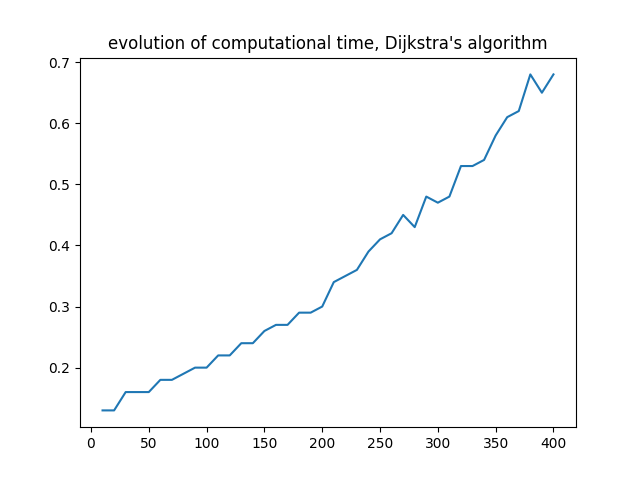
\includegraphics[width=7.5cm]{ressources/dijkstra_res_graph.png}
	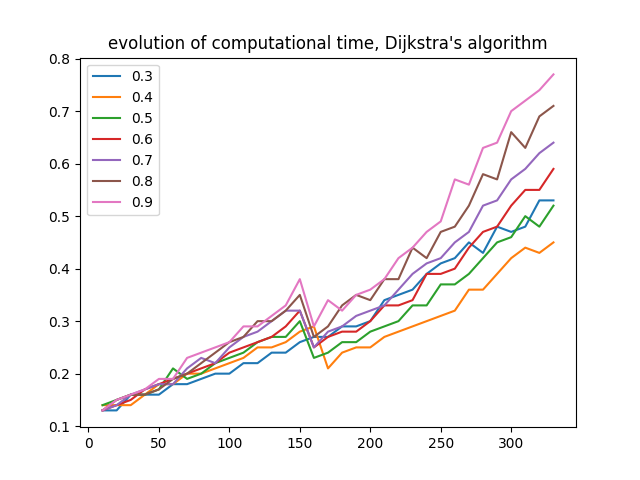
\includegraphics[width=7.5cm]{ressources/dijkstra_res_graph_density.png}
	\caption{dijkstra\_graph}
	\label{fig:dijkstra}
\end{figure}

First, here (figure ~\ref{fig:dijkstra}) is the evolution of computational time for Dijkstra's on the
structure ``Graph'':

To obtain the figure (figure ~\ref{fig:dijkstra}), the algorithm was run on graphs of 10 to 400 nodes. The figure on the left shows the evolution at a given density, while the one on the right shows the evolution with different densities.

It can be noted that for densities over .6, computation time increases with density, which can be expected. But for densities lower than that, there is no consensus. No matter the density, it increases gradually with the size, which is very logical. It can be thought that for densities too small, the data structure is such that it does change much to have a lower density. There is some kind of threshold effect, at which the unadapted structure overcomes the density variation.

Dijkstra's algorithm has a $\mathcal O(e+v\log(v))$ complexity, where $e$ is the number of edges and $v$ the number of vertices. The curves obtained are not unlike that complexity of $v\log(v)$. Though the prefactor is unknown and the number of vertices in the graph stayed relatively small in my tests (max 400). It was already sufficient for my computer to run for quite some time

\begin{figure}[!h]
	\centering
	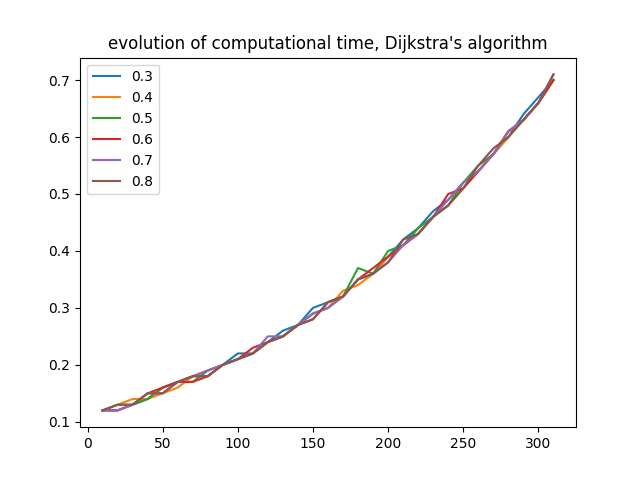
\includegraphics[width=7.5cm]{ressources/dijkstra_density_std_graph.png}
	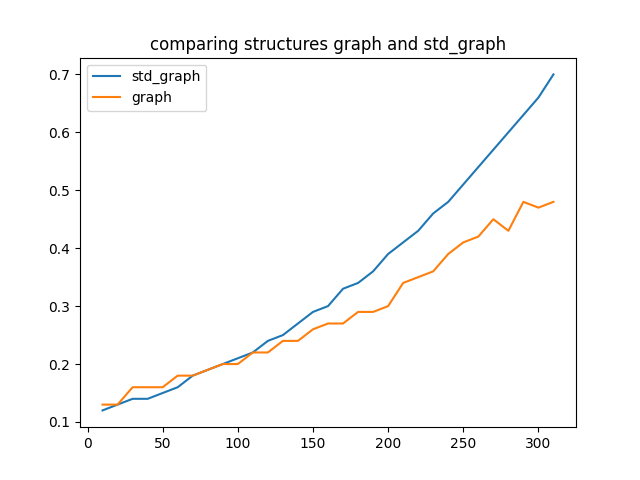
\includegraphics[width=7.5cm]{ressources/comparing_graph__std_graph.png}
	\caption{structure std\_graph}
	\label{fig:stdgraph}
\end{figure}

Now, let's see the Structure ``std\_graph``. First alone at different densities, then it can be compared to the results obtained with \texttt{graph} (figure ~\ref{fig:stdgraph}).

It can be seen that \texttt{std\_graph} tends to be slower as the number of nodes (and hence arcs) increases. That's probably due to the fact that the algorithm is very similar, but the data structure is larger when the density is big. The structure is less memory-efficient for large densities. 


\begin{figure}[!h]
	\centering
	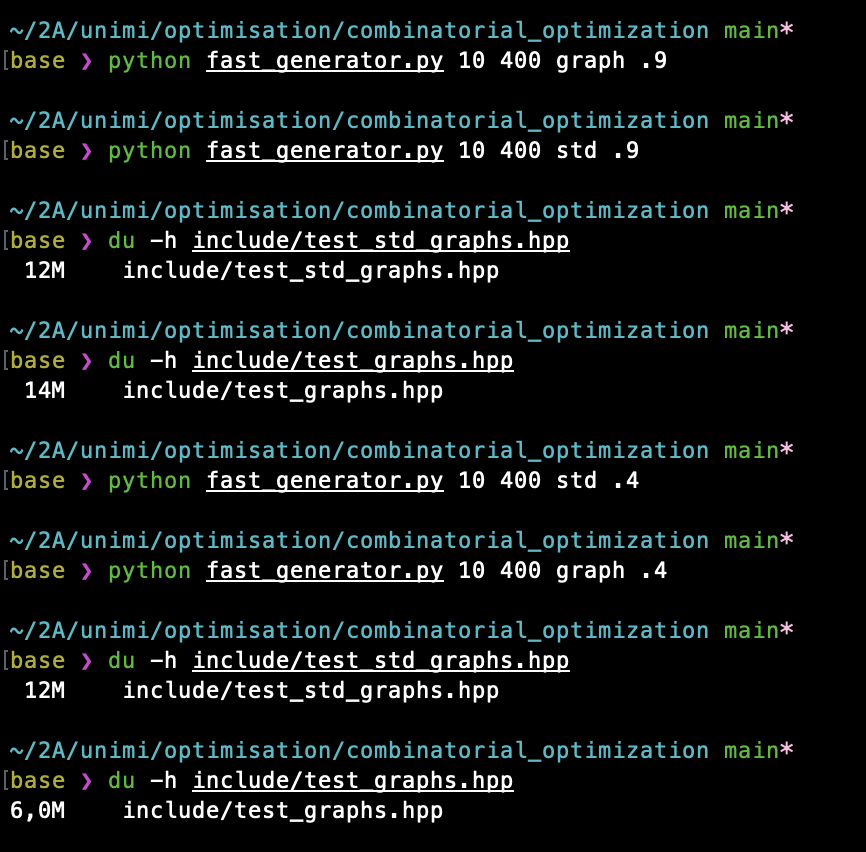
\includegraphics[width=9cm]{ressources/spatial_comp.png}
	\caption{comparing\_size}
	\label{fig:sizecomparizon}
\end{figure}

To check that hypothesis, let's compare the size of the files containing structures \texttt{graph} and \texttt{std\_graph} at two different densities (figure ~\ref{fig:sizecomparizon}).

As expected, the files are very similar when the density is high. \texttt{std\_graph} always has the same size and is hence more relevant for \textbf{high densities}. On the contrary, when the density is low, \texttt{std\_graph} contains lots of zeros, whereas \texttt{graph} only keeps the \textbf{relevant} information. That's why \texttt{std\_graph} takes up twice as much space on low densities.

\hfill
\hfill
\hfill

A point on \textbf{methodology}: to run the tests, I wrote some shell scripts to automatize the tasks of varying densities and number of vertices. To have good results, I ran each combination of density and number of vertices 10 times and computed the mean time of this, so as to reduce measuring uncertainty as much as possible. I also shut down all other activities on my computer so as to avoid noise on the measures. This way, I hope that the results are as precise as possible and reflect the reality of the algorithm's performance.

\section{Thanks}

I would like to thank Professor Giovanni Righini for his very interesting class. Coming from France, I had the opportunity to attend an Erasmus+ exchange in Milan and learned lots from it. The University of Milan was very well organised and the classes very challenging. 

\newpage

\section{Appendix}

\subsection{Source Code}

All the source code is available on github: \href{https://www.github.com/plgstalter/combinatorial_optimization}{github.com/plgstalter/combinatorial\_optimization}.

For the sake of simplicity, I will just present the organization of the files.

\begin{figure}[htp]
	\centering
	\includegraphics[width=6cm]{ressources/tree_dij.png}
	\hfill
	\includegraphics[width=6cm]{ressources/tree_kru.png}
	\caption{Organization of source files for Dijkstra (left) and Kruskal (right)}
\end{figure}

The structure is pretty simple.

\newpage

And the makefiles as well:

\begin{multicols}{2}

For Dijkstra:

\begin{verbatim}
CC=g++
CFLAGS= -std=c++17 -Wall -ggdb -Iinclude

src := $(wildcard src/*.cpp)
obj := $(subst src, build, $(src:.cpp=.o))

.PHONY: directories

all: directories project
	@echo $(obj)

project: main.o build
	$(CC) $(CFLAGS) -o project main.o build/*.o

main.o: main.cpp $(obj)
	$(CC) $(CFLAGS) -c main.cpp

build/%.o: src/%.cpp include/%.h
	$(CC) $(CFLAGS) -o $@ -c $<

directories: build
build:
	mkdir -p $@

clean:
	rm -r build
	rm main.o
	rm include/*.gch
\end{verbatim}

\columnbreak

And for Kruskal:

\begin{verbatim}
.PHONY: directories

all: project

project: main.o kruskal.o
	g++ -o project main.o kruskal.o

main.o: main.cpp kruskal.h
	g++ -c main.cpp

kruskal.o: kruskal.cpp
	g++ -c kruskal.cpp

clean:
	rm *.o
	rm project

\end{verbatim}
\end{multicols}
\end{document}

